\documentclass[openany,12pts,letterpaper,oneside,onecolumn]{book}

\usepackage[utf8]{inputenc}
\usepackage[spanish]{babel}
\usepackage{graphicx}
\usepackage{float}
\usepackage[hidelinks]{hyperref}
\usepackage{amssymb}
\usepackage{listings}
\usepackage{booktabs}
\usepackage{multirow}
\usepackage[table,xcdraw]{xcolor}
\usepackage{lscape}
\usepackage{longtable}


%codigo en java
\lstdefinestyle{customc}{
	belowcaptionskip=1\baselineskip,
	breaklines=true,
	frame=L,
	xleftmargin=\parindent,
	language=Java,
	showstringspaces=false,
	basicstyle=\footnotesize\ttfamily,
	keywordstyle=\bfseries\color{green!40!black},
	commentstyle=\itshape\color{purple!40!black},
	identifierstyle=\color{blue},
	stringstyle=\color{orange},
}
\lstdefinestyle{customasm}{
	belowcaptionskip=1\baselineskip,
	frame=L,
	xleftmargin=\parindent,
	language=[x86masm]Assembler,
	basicstyle=\footnotesize\ttfamily,
	commentstyle=\itshape\color{purple!40!black},
}

\lstset{escapechar=@,style=customc}

%parrafos
\makeatletter
\newcounter{subsubparagraph}[subparagraph]
\renewcommand\thesubsubparagraph{%
	\thesubparagraph.\@arabic\c@subsubparagraph}
\newcommand\subsubparagraph{%
	\@startsection{subsubparagraph}    % counter
	{6}                              % level
	{\parindent}                     % indent
	{3.25ex \@plus 1ex \@minus .2ex} % beforeskip
	{-1em}                           % afterskip
	{\normalfont\normalsize\bfseries}}
\newcommand\l@subsubparagraph{\@dottedtocline{6}{10em}{5em}}
\newcommand{\subsubparagraphmark}[1]{}
\makeatother
\setcounter{tocdepth}{5}
\setcounter{secnumdepth}{5}


\begin{document}

\author{  Daniela Córdoba Acosta\\
	Johan Quiroga Torres\\
	Santiago Jiménez Bonilla
}
\title{	TWO WHEELS PARKING\\
	Sistema de Gestión de biciparqueaderos}

\date{Febrero 2018}

\frontmatter
\maketitle
\tableofcontents

\mainmatter

\part{Contexto}
\chapter{Proyecto}

\section{Objetivos del Proyecto} 

\subsection{Objetivo General} 
Automatizar y optimizar los principales procesos realizados por el sistema actual de parqueaderos para bicicletas de la empresa Two Wheels Parking. Además de implementar herramientas informáticas pertinentes a las necesidades de quienes quieren hacer uso de este servicio, mejorando así, su calidad como usuarios activos del servicio. 

\subsection{Objetivos Específicos}
\begin{itemize}
	\item Optimizar los principales procesos que hacen parte del propósito de brindar servicios de parqueo para las bicicletas en las diferentes sucursales que maneja Two Wheels Parking, a través de una planeación y modelamiento de dichos procesos con el fin de mejorar el uso de los espacios destinados al almacenamiento de bicicletas.
	\item Automatizar los procesos de registro y consulta de información pertinente, a través de la elaboración de herramientas información con el propósito de incrementar la eficiencia del servicio de biciparqueaderos de la organización.
	\item Generar un software confiable, robusto y escalable, por medio de la elaboración de modelos utilizando como herramienta los patrones de diseño de software, para mejorar el sistema actual de manejo de parqueaderos y realizar aportes a futuras mejoras a dicho sistema.
\end{itemize}

%\cite{LBol,AIsh,ATak}

\chapter{Metodologia}

\part{Arquitecura}
\chapter{Organizacion}

\begin{figure}[H]
	\centering
	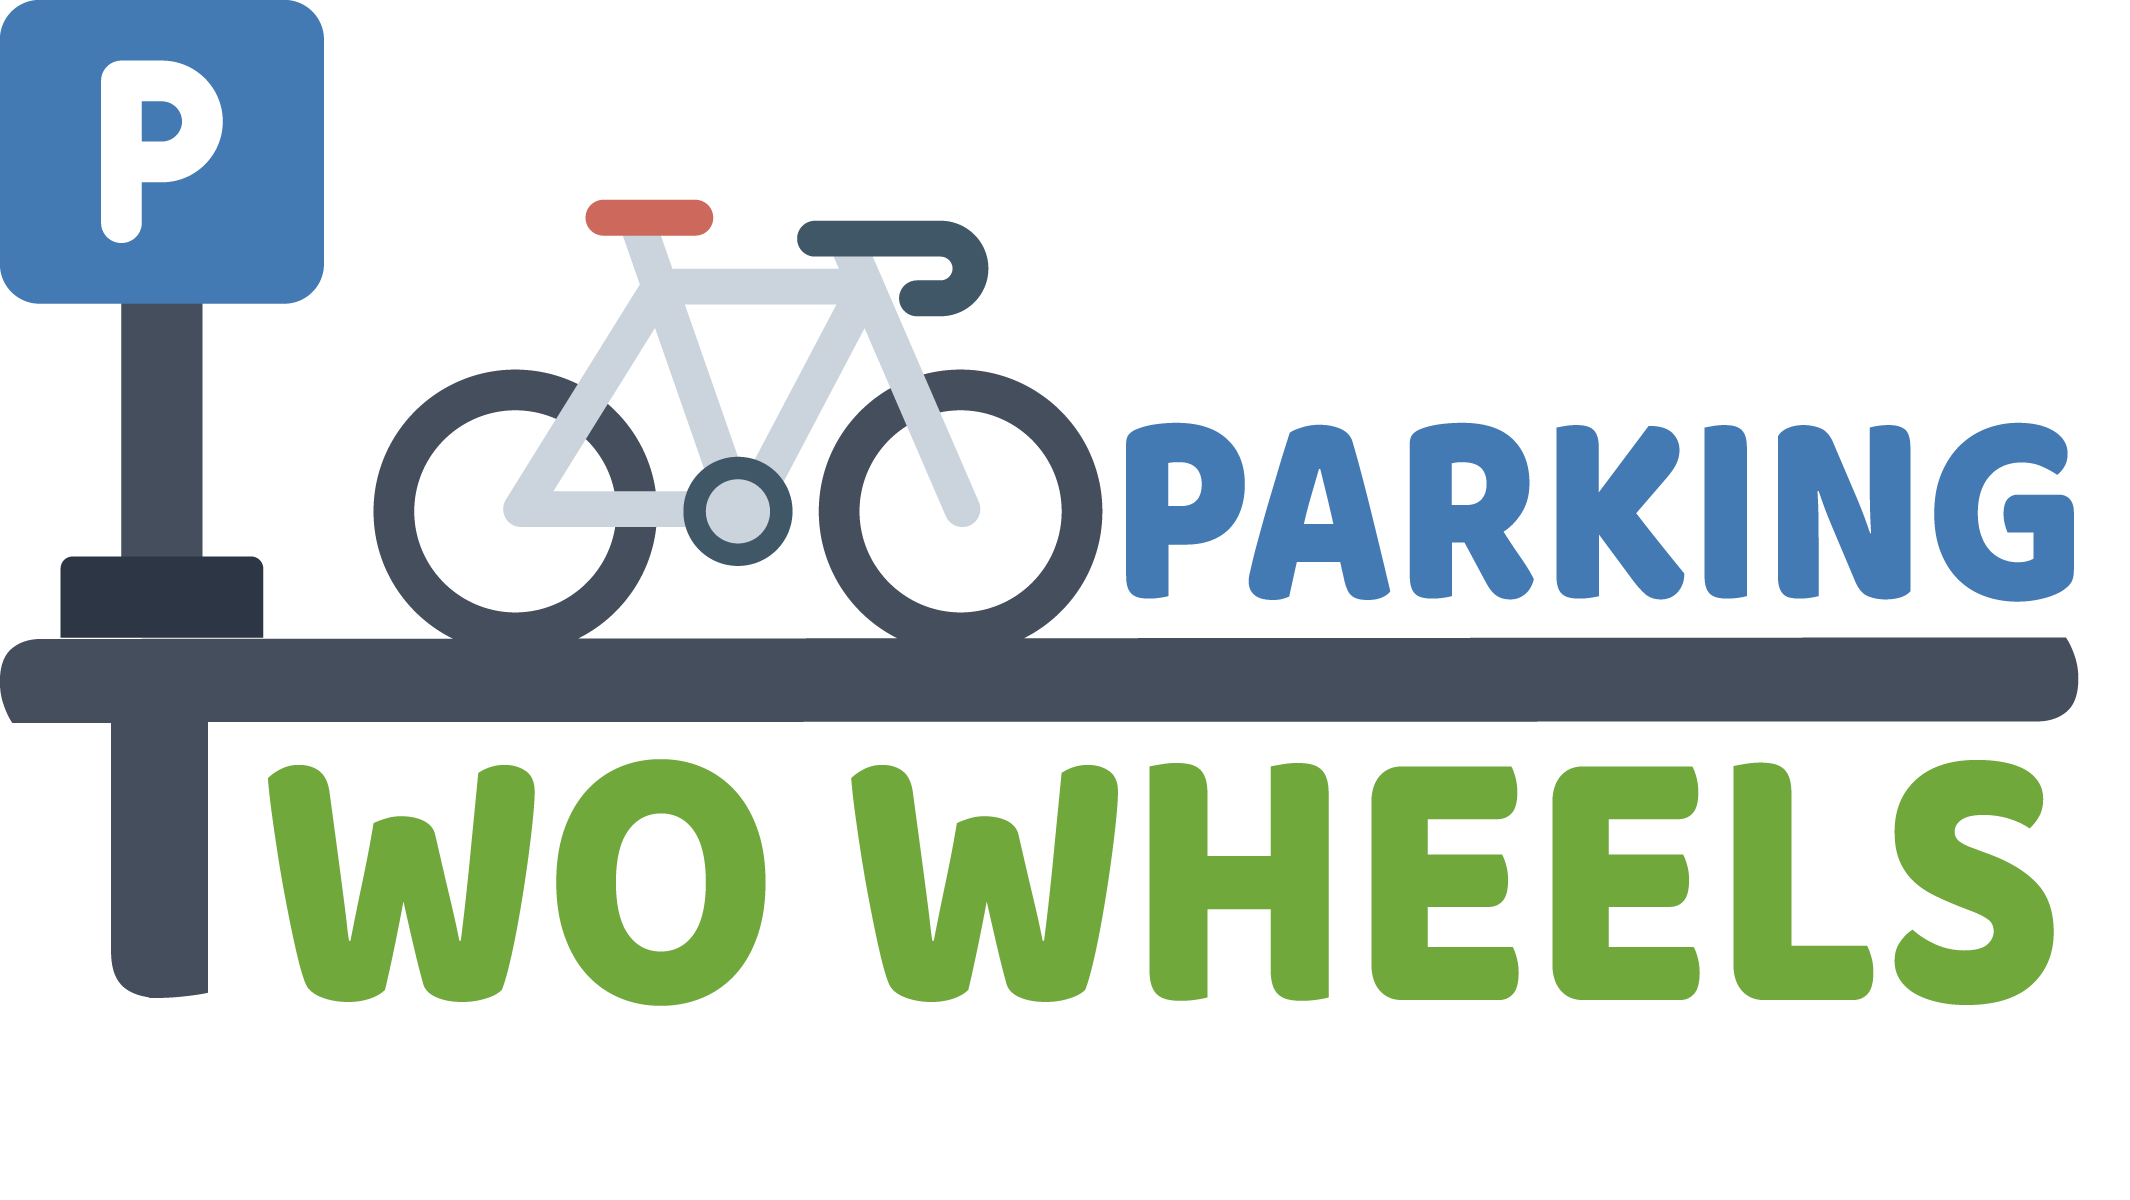
\includegraphics[scale=0.5]{imagenes/logoTWP}
	\caption{Two Wheels Parking}
	\label{fig:logotwp}
\end{figure}


\section{Misión}
En Two Wheels Parking ofrecemos soluciones de aparcamiento para bicicletas en la ciudad de Bogotá, ofreciendo una experiencia de tranquilidad, seguridad y organización a nuestros clientes,  buscando incentivar el uso de este medio de transporte como una alternativa limpia y segura.\\

\section{Visión}
Queremos estar comprometidos con los problemas de nuestros clientes de forma transparente y eficaz, convirtiéndonos en un socio de confianza. En Two Wheels Parking queremos ser un referente como una empresa líder en soluciones de aparcamiento, dando a conocer nuestra marca como una empresa ética, responsable y solidaria con nuestros clientes.\\

\section{Estructura Organizacional}
\begin{figure}[H]
	\centering
	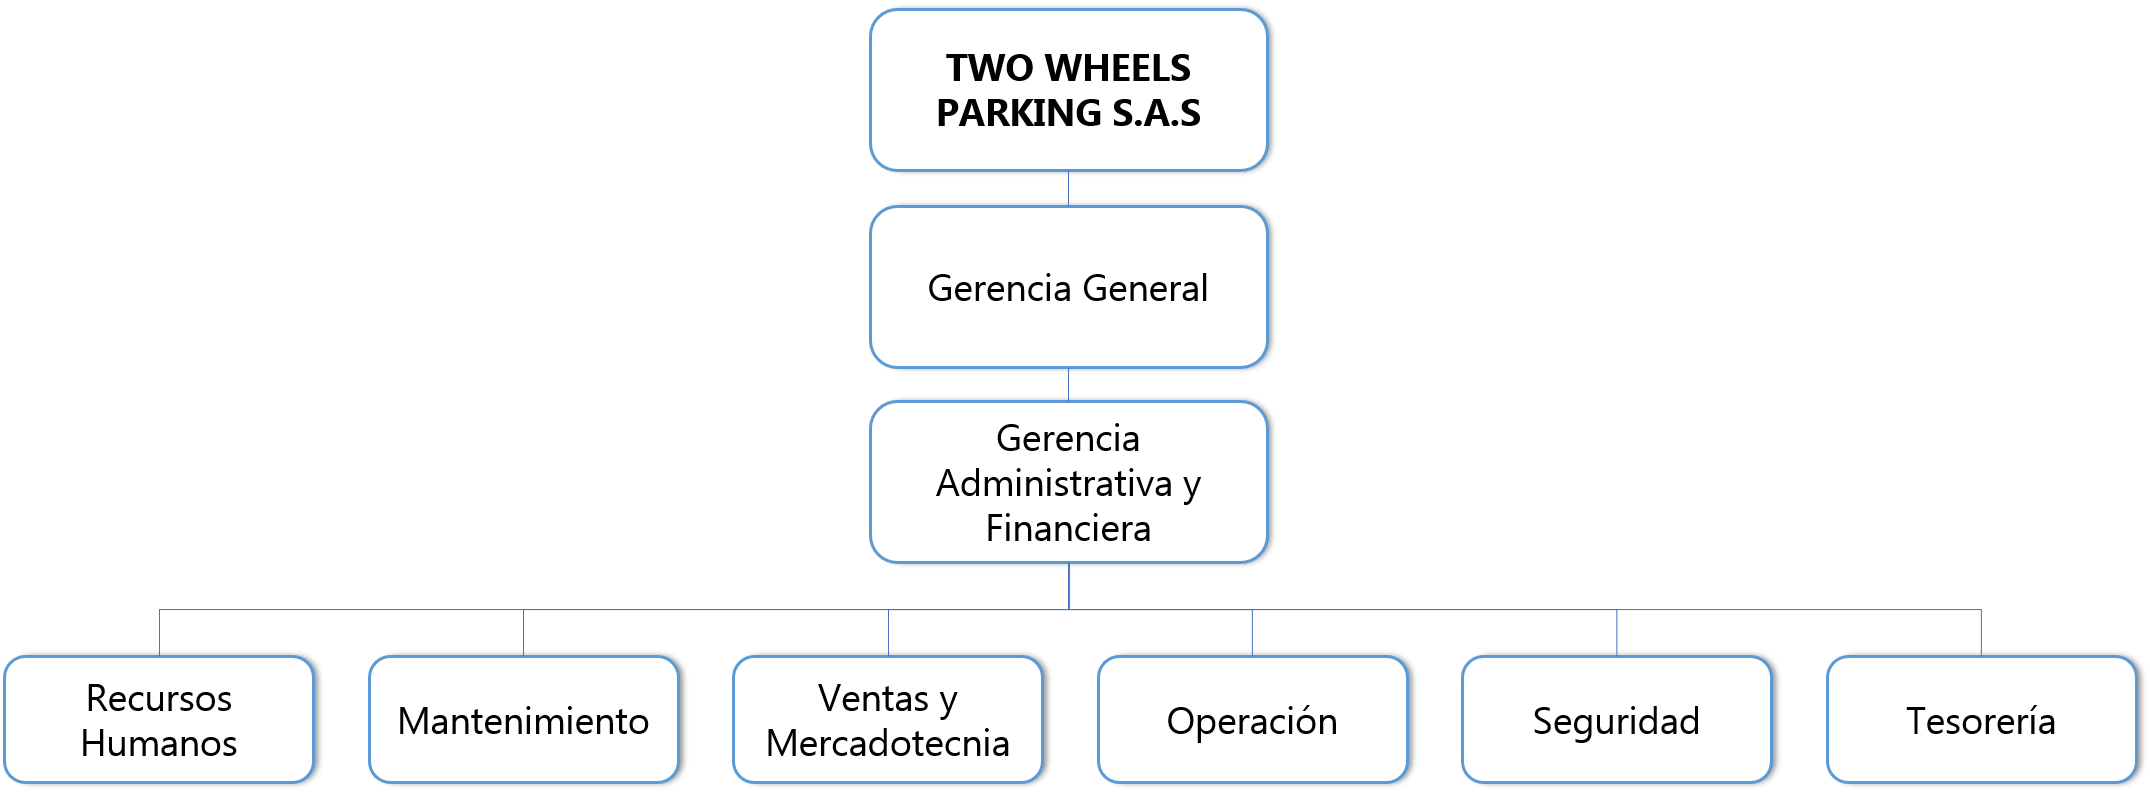
\includegraphics[width=0.7\linewidth]{imagenes/organigrama}
	\caption{Organigrama General de Two Wheels Paking.}
	\label{fig:organigrama}
\end{figure}

\section{Funciones de Negocio y Manual de funciones}

\subsubsection {Recursos humanos}
\begin{itemize}
	\item Trabajadora social: Profesional encargado del desarrollo de vínculos humanos saludables y buenas relaciones sociales entre los individuos que laboran al interior de la empresa.\\
\end{itemize}

\subsubsection {Gerencia}
\begin{itemize}
	\item Presidente: Representante, líder y supervisor en la toma de decisiones que guían el rumbo de la compañía. \\
	\item Secretaria: Principal colaboradora del presidente en el área administrativa, dentro de su rol es la encargada de la gestión de la documentación empresarial y de la atención al público.\\
\end{itemize}

\subsubsection{Seguridad} 
\begin{itemize}
	\item Guardia de seguridad: personal competente para realizar  actividades  de  vigilancia,  inspección,  prevención  y  detección  de  anormalidades  al interior de la Institución.
\end{itemize}

\subsubsection{Tesorería} 
\begin{itemize}
	\item Tesorero: Encargado de gestionar y dirigir los asuntos relacionados con movimientos económicos o flujos monetarios, tanto captación como desembolsos dentro de la empresa.
\end{itemize}

\subsubsection{Administrativo y contable} 
\begin{itemize}
	\item Contador Público: Profesional encargado de realizar y verificar los registros contables, tributarios y financieros de la empresa, generando los informes y documentos legales exigidos por la legislación nacional.
	\item Administrador: Responsable de la gestión de recursos materiales y financieros dedicados a la realización y control de las distintas actividades tanto técnica como administrativas mediante una correcta planificación, coordinación y ejecución.
\end{itemize}

\subsubsection{Ventas y mercadotecnia}
\begin{itemize}
	\item Agentes de ventas: Profesionales capaces de captar y aumentar el número y la calidad de clientes a los cuales la empresa busca prestar una serie de soluciones.
	\item Publicista: Experto en supervisar, coordinar y ejecutar estrategias de publicidad y posicionamiento de imagen tanto de la empresa como de los productos que se generan al interior de ella.
\end{itemize}


\section{Procesos de Negocio}
\begin{figure}[H]
	\centering
	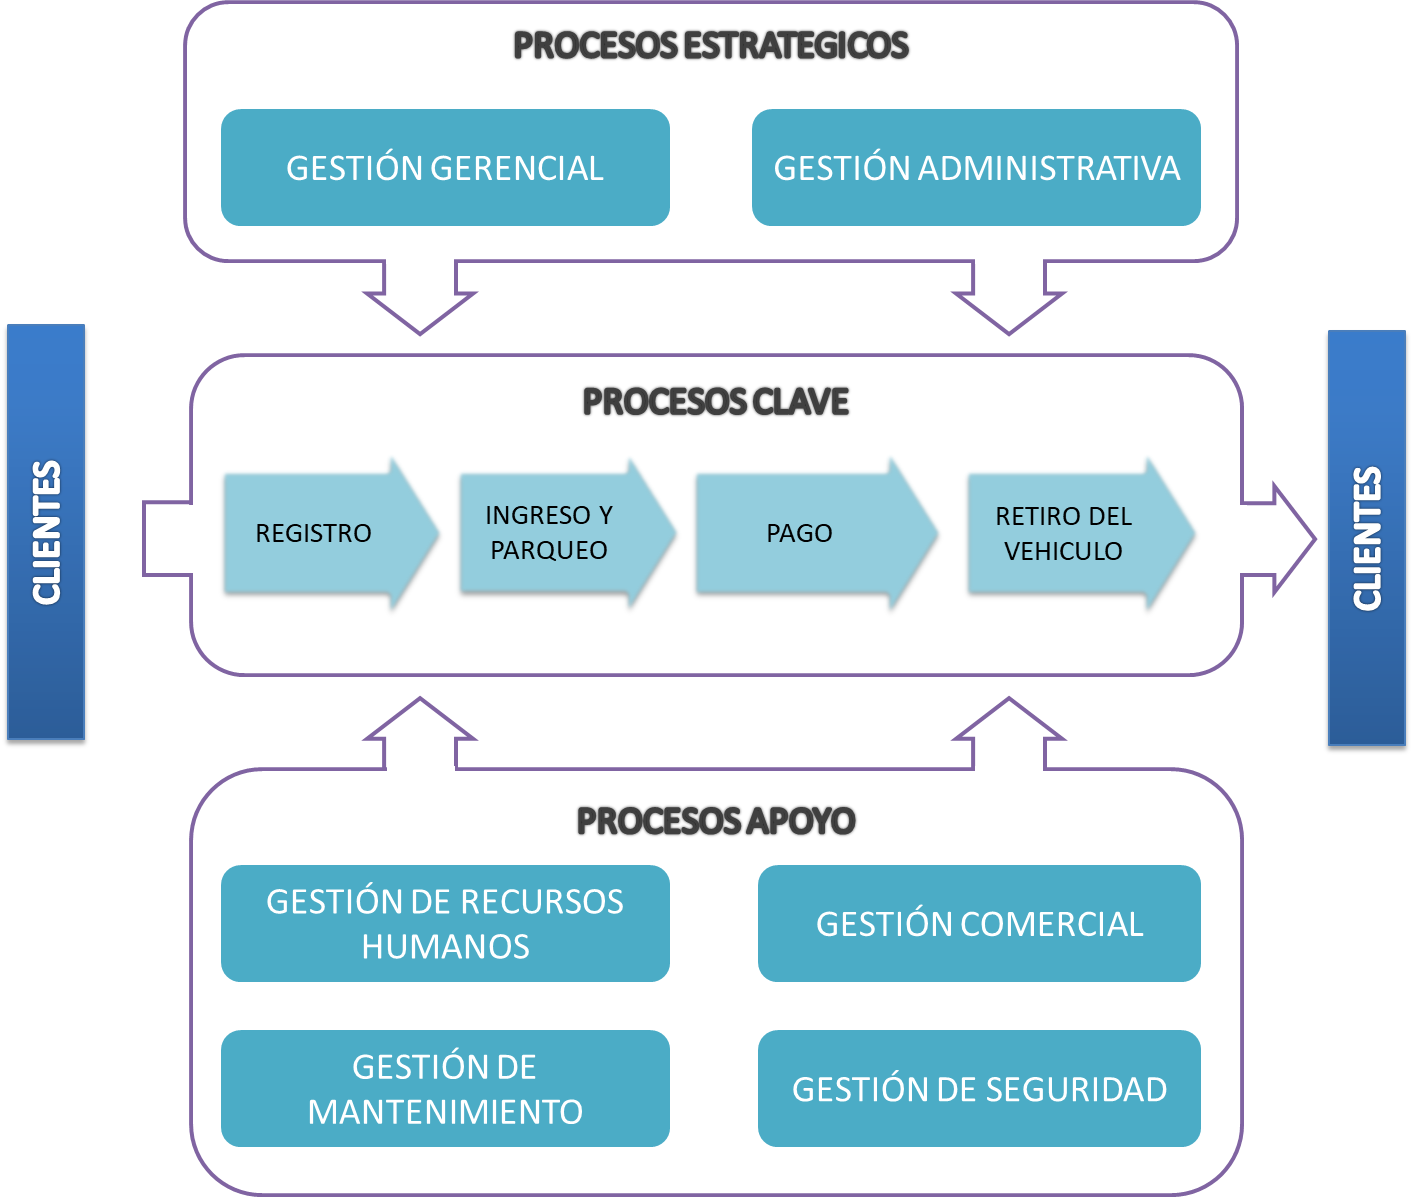
\includegraphics[width=0.8\textwidth]{imagenes/mapProcTWP}
	\caption{Mapa de Procesos de Two Wheels Paking.}
	\label{fig:awesome_image}
\end{figure}

\section{Objetivos}
\subsection{Organizacionales}
\begin{itemize}
	\item Alcanzar un amplio mercado a nivel nacional convirtiéndonos en una de las empresas pioneras de soluciones en colaboración con el medio ambiente, brindando soluciones de parqueo a aquellas personas que hacen uso de un transporte ecológico, esto con el fin de fomentar el uso de dicho transporte y contribuir al desarrollo sustentable.
\end{itemize}

\subsection{Operacionales}
\begin{itemize}
	\item Brindar la mejor calidad de servicio a nuestros clientes, mediante un equipo de trabajo altamente capacitado, convirtiéndonos en una de las empresas distritales con uno de los mejores “Goodwill”.
\end{itemize}

\subsection{Misionales}
\begin{itemize}
	\item Enfocar todos nuestros procesos al uso eficiente de los insumos y recursos, esto mediante el fomento de responsabilidad social tanto al interior como al exterior de la empresa en nuestros empleados, generando así un Impacto ambiental positivo a partir de la producción de nuestros productos y servicios.
\end{itemize}

\subsection{Estratégicos}
\begin{itemize}
	\item Posicionar a la empresa y su marca Two Wheels como una franquicia respetable de parqueo, esto mediante la estandarización y normalización de nuestros procesos, estableciendonos y generando un impacto primeramente a nivel distrital y posteriormente nacional.
\end{itemize}

\section{Valores Organizacionales}
\subsection{Amabilidad:}  En Two Wheels queremos prestar un servicio de calidad al cliente, por lo cual contamos con un equipo de trabajo capacitado el cual atenderá sus inquietudes y propuestas de la mejor manera.
\subsection{Cumplimiento:}
Sabemos que el tiempo y el dinero son recursos importantes, por eso en Two Wheels nos regimos bajo estrictos estándares y políticas internas para que las actividades estipulados se lleven a cabo en los tiempos predefinidos, los que nos convierte en una empresa sólida y seria de cara a nuestros clientes.
\subsection{Seguridad:}
En Two Wheels nos comprometemos con nuestros usuarios para brindar un ambiente seguro para sus vehículos mediante un control de acceso de usuarios efectivo e instalaciones que cuenten con una infraestructura adecuada para proteger a cada usuario y su vehículo.
\subsection{Respeto:}
En Two Wheels creemos que el pilar de toda organización es el respeto mutuo. Por eso, nuestro equipo está enfocado en brindar el mejor servicio a todos nuestros clientes, sin ninguna excepción.
\subsection{Honestidad:}
Como parte de nuestra misión, en Two Wheels creemos en el manejo transparente de nuestros procesos, ofreciendo a nuestros clientes un servicio en el cual puedan confiar.


\chapter{Achimate -ADM}

El método ADM y en general el marco TOGAF realiza el análisis arquitectónico con alto nivel de abstracción para visualizar, detectar y
	documentar oportunidades y riesgos durante el desarrollo de la arquitectura, direccionando la arquitectura empresarial con la ayuda de sus herramientas.
TOGAF esta compuesto por 3 partes principales el método de desarrollo ADM (Architecture Development Method), la taxonomía empresarial (Enterprise Continuum) y la base de recursos (Architecture Repository). Aborda el desarrollo a partir de 4 niveles de abstracción:
\begin{itemize}
	\item Arquitectura de Negocio
	\item Arquitectura de Aplicación
	\item Arquitectura de Datos
	\item Arquitectura Tecnológica
\end{itemize}
ADM muestra estos niveles de abstracción en diferentes fases que determinan la linea base (baseline) y el final del nivel de abstracción (target), donde el analisis de brecha (gap analysis - figura 5.1) permite conocer el estado final de la arquitectura despues de una o varias iteraciones.
\begin{figure}[H]
	\centering
	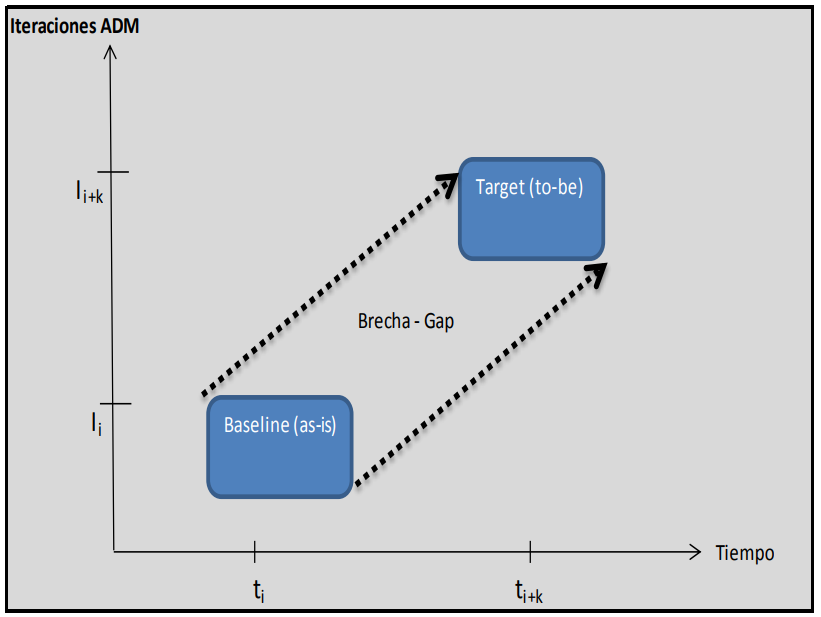
\includegraphics[width=1.0\textwidth]{imagenes/Captura.PNG}
	\caption{Analisis de Brecha -Iteraciones ADM}
	\label{fig:gap_analysis}
\end{figure}

Este análisis mide los objetivos de arquitectura y el grado de la madurez alcanzados por la organización

ADM consta de 8  niveles o etapas y un paso preliminar donde se describen las actividades iniciales, principios y capacidades de la arquitectura objetivo, también se realiza una adaptación del marco de trabajo para ajustarlo a las necesidades de la organización.
\cite{FGuti}

\begin{figure}[H]
	\centering
	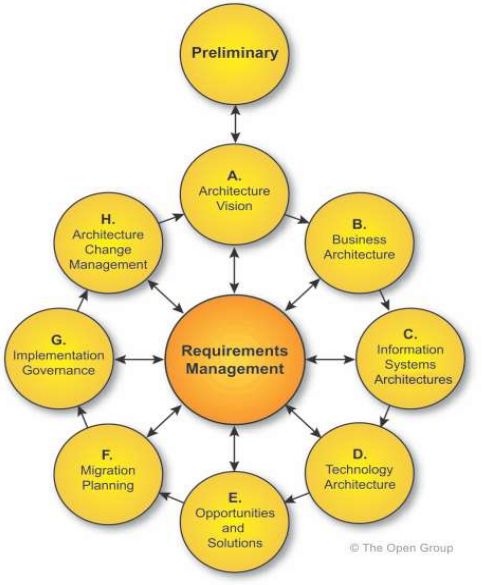
\includegraphics[width=1.0\textwidth]{imagenes/Captura1.PNG}
	\caption{Etapas del Método ADM}
	\label{fig:gap_analysis}
\end{figure}

Las primeras cuatro fases definen los niveles de abstracción antes mencionados para el desarrollo de la arquitectura, la fase E de la interacción define oportunidades y soluciones que se deben implementar.

Estas oportunidades y soluciones se identifican e incluyen en el plan de migración, fase F. En esta fase se desarrolla el producto de software con los requerimientos y especificaciones obtenidos de las anteriores fases, luego lleva a su implementación (fase G) y como finalidad lleva la arquitectura de un estado base (baseline) al estado objetivo (target), estas dos fases dan gobernabilidad y gestión de control de cambios a la arquitectura. Este ciclo se repite hasta llegar a la vision establecida en la fase preliminar junto con la vision inicialmente concebida.


\section{TOGAF}
\subsection{Resumen: capa de negocio}

\begin{center}
	\begin{longtable}[H]{|p{5cm}|p{6cm}|p{3cm}|}
		\hline
		\textbf{Concepto} &  \centering \textbf{Definición} & \textbf{Notación} \\
		\hline
		\endfirsthead
		
		
		\hline
		\textbf{Concepto} &  \centering \textbf{Definición} & \textbf{Notación} \\
		\hline
		\endhead
		
		%inicio contenido tabla 
		
		\centering \textbf{Actor de negocio}\\ \textbf{(Business actor)} & Una entidad organizativa que es capaz de realizar el comportamiento.         & 
		\raisebox{-\totalheight}{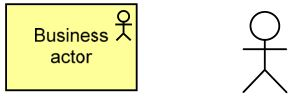
\includegraphics[scale=0.36]{imagenes/lenguaje/Bussines/actor}}\\ 		\hline         
		
		
		\centering \textbf{Papel del negocio}\\ \textbf{(Business role)} & La responsabilidad de realizar un comportamiento específico, al cual un actor puede ser asignado.&\raisebox{-\totalheight}{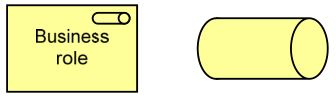
\includegraphics[scale=0.36,]{imagenes/lenguaje/Bussines/role}}\\
		\hline
		
		
		\centering \textbf{Colaboración Empresarial}\\ \textbf{(Business Collaboration)} & Un agregado de dos o más funciones empresariales que trabajan juntas para realizar un comportamiento colectivo. &  \raisebox{-\totalheight}{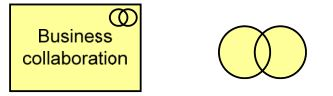
\includegraphics[scale=0.36,] {imagenes/lenguaje/Bussines/collaboration}}\\ 
		\hline
		
		
		\centering \textbf{Interfaz de negocios}\\ \textbf{(Business interface)} & Un punto de acceso donde un servicio comercial está disponible para el medio ambiente..&  \raisebox{-\totalheight}{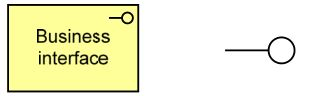
\includegraphics[scale=0.36,]{imagenes/lenguaje/Bussines/interface}}\\ 
		\hline
		
		\centering \textbf{Ubicación}\\ \textbf{(Location)}& Un punto conceptual o extensión en el espacio.&  
		\raisebox{-\totalheight}{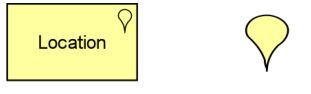
\includegraphics[scale=0.36,]{imagenes/lenguaje/Bussines/location}}\\ 
		\hline
		
		\centering \textbf{Objeto de negocio}\\ \textbf{(Business Object)}& Un elemento pasivo que tiene relevancia desde una perspectiva empresarial.&  
		\raisebox{-\totalheight}{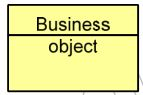
\includegraphics[scale=0.36,]{imagenes/lenguaje/Bussines/object}}\\ 
		\hline
		
		\centering \textbf{Proceso de negocio}\\ \textbf{(Business Process)}& Un elemento de comportamiento que agrupa el comportamiento basado en un ordenamiento de actividades. Se pretende producir un conjunto definido de productos o servicios empresariales.&  
		\raisebox{-\totalheight}{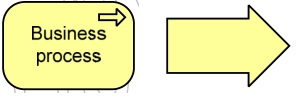
\includegraphics[scale=0.36,]{imagenes/lenguaje/Bussines/process}}\\ 
		\hline
		
		\centering \textbf{Función de negocio}\\ \textbf{(Business Function)}& Un elemento de comportamiento que agrupa el comportamiento basado en un conjunto seleccionado de criterios (normalmente requeridos por los recursos empresariales y / o las competencias).&  
		\raisebox{-\totalheight}{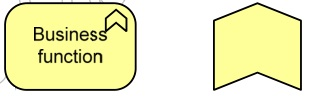
\includegraphics[scale=0.36,]{imagenes/lenguaje/Bussines/funtion}}\\ 
		\hline
		
		\centering \textbf{Interacción de negocios}\\ \textbf{(Business Interaction)}& Un elemento de comportamiento que describe el comportamiento de una colaboración comercial.&  
		\raisebox{-\totalheight}{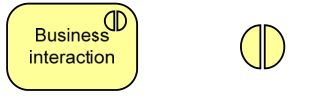
\includegraphics[scale=0.36,]{imagenes/lenguaje/Bussines/interaction}}\\ 
		\hline
		
		\centering \textbf{Evento de negocios}\\ \textbf{(Business Event)}& Algo que sucede (internamente o externamente) e influye en el comportamiento.&  
		\raisebox{-\totalheight}{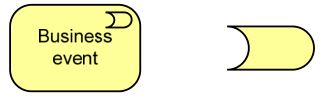
\includegraphics[scale=0.36,]{imagenes/lenguaje/Bussines/event}}\\ 
		\hline
		
		\centering \textbf{Servicio de negocio o empresarial}\\ \textbf{(Business Service)}& Un servicio que satisface una necesidad de negocio para un cliente (interno o externo a la organización).&  
		\raisebox{-\totalheight}{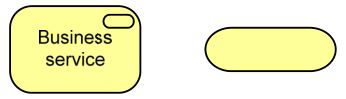
\includegraphics[scale=0.36,]{imagenes/lenguaje/Bussines/service}}\\ 
		\hline
		
		\centering \textbf{Representación}\\ \textbf{(Representation)}& Una forma perceptible de la información transportada por un objeto de negocio.&  
		\raisebox{-\totalheight}{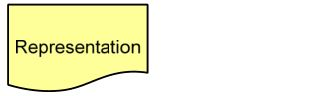
\includegraphics[scale=0.36,]{imagenes/lenguaje/Bussines/representation}}\\ 
		\hline
		
		\centering \textbf{Significado}\\ \textbf{(Meaning)}& Los conocimientos o experiencia presentes en un objeto de negocio o su representación, dado un contexto particular.&  
		\raisebox{-\totalheight}{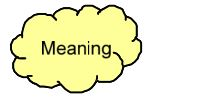
\includegraphics[scale=0.36,]{imagenes/lenguaje/Bussines/meaning}}\\ 
		\hline
		
		\centering \textbf{Valor}\\ \textbf{(Value)}& El valor relativo, la utilidad o la importancia de un servicio o producto comercial.&  
		\raisebox{-\totalheight}{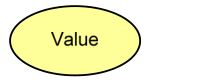
\includegraphics[scale=0.36,]{imagenes/lenguaje/Bussines/value}}\\ 
		\hline
		
		
		\centering \textbf{Producto}\\ \textbf{(Product)}& Un conjunto coherente de servicios, acompañado de un contrato / conjunto de acuerdos, que se ofrece en su conjunto a clientes (internos o externos).&  
		\raisebox{-\totalheight}{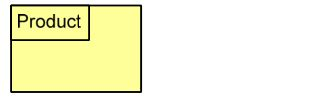
\includegraphics[scale=0.36,]{imagenes/lenguaje/Bussines/product}}\\ 
		\hline
		
		
		\centering \textbf{Contrato}\\ \textbf{(Contract)}& Una especificación formal o informal de acuerdo que especifica los derechos y obligaciones asociados con un producto.&  
		\raisebox{-\totalheight}{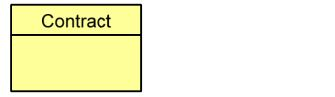
\includegraphics[scale=0.36,]{imagenes/lenguaje/Bussines/contract}}\\ 
		\hline
		
		\caption{Capa de Negocio}
		\label{capa-business}
	\end{longtable}
\end{center}

\subsection{Resumen: capa de aplicación}
\begin{table}[H]
	\centering
	\begin{tabular}{|p{5cm}|p{6cm}|p{3.3cm}|}
		\hline
		\textbf{Concepto}                                                           & \multicolumn{1}{c|}{\textbf{Definición}}                                                             & \textbf{Notación} \\ \hline
		\begin{tabular}[c]{@{}c@{}}\textbf{Componente de Aplicación}\\ \textbf{(Application Component)}\end{tabular} & Una parte modular, desplegable y reemplazable de un sistema de software que encapsula su comportamiento y datos y los expone a través de un conjunto de interfaces.    & 	\raisebox{-\totalheight}{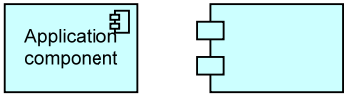
\includegraphics[scale=0.36,]{imagenes/lenguaje/Aplication/componentApp}}
		\\ \hline
		\begin{tabular}[c]{@{}c@{}}\textbf{Colaboración de Aplicación}\\ \textbf{(Application
				collaboration)}\end{tabular}            & 
		Un agregado de dos o más componentes de aplicación que trabajan juntos para realizar un comportamiento colectivo.                         & 
		\raisebox{-0,63\totalheight}{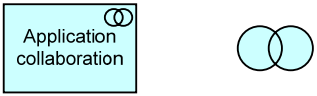
\includegraphics[scale=0.28,]{imagenes/lenguaje/Aplication/collaborationApp}}   \\ \hline
		\begin{tabular}[c]{@{}c@{}}\textbf{Interfaz de Aplicación}\\ \textbf{(Application interface)}\end{tabular}                  & Un punto de acceso donde un servicio de aplicación está disponible para un usuario u otro componente de aplicación &  \raisebox{-0,63\totalheight}{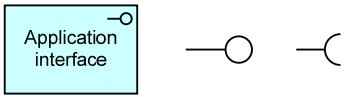
\includegraphics[scale=0.36,]{imagenes/lenguaje/Aplication/interfaceApp}} 
		\\ \hline
		\begin{tabular}[c]{@{}c@{}}\textbf{Objeto de Datos}\\ \textbf{(Data Object)}\end{tabular}                      & Un elemento pasivo adecuado para el procesamiento automatizado.                                  & 
		\raisebox{-0,63\totalheight}{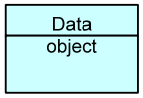
\includegraphics[scale=0.36,]{imagenes/lenguaje/Aplication/dataObjectApp}}
		\\ \hline
		\begin{tabular}[c]{@{}c@{}}\textbf{Función de Aplicación}\\ \textbf{(Function Application)}\end{tabular}                      & 
		Un elemento de comportamiento que agrupa el comportamiento automatizado que puede ser realizado por un componente de aplicación.                                & \raisebox{-0,63\totalheight}{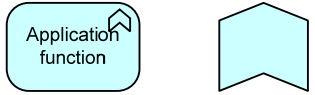
\includegraphics[scale=0.36,]{imagenes/lenguaje/Aplication/functionApp}}
		\\ \hline
		\begin{tabular}[c]{@{}c@{}}\textbf{Interacción de Aplicación}\\ \textbf{(Application
				interaction)}\end{tabular}                      & 
		Un elemento de comportamiento que describe el comportamiento de una colaboración de aplicación                                  & 
		\raisebox{-0,63\totalheight}{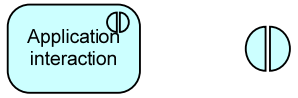
\includegraphics[scale=0.36,]{imagenes/lenguaje/Aplication/interactionApp}}
		\\ \hline
		\begin{tabular}[c]{@{}c@{}}\textbf{Servicio de Aplicación}\\ \textbf{(Application
				Service)}\end{tabular}                      & 
		Un servicio que expone un comportamiento automatizado                                 & \raisebox{-0,63\totalheight}{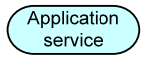
\includegraphics[scale=0.36,]{imagenes/lenguaje/Aplication/serviceApp}}
		\\ \hline
	\end{tabular}
	\caption{Capa de Aplicación}
	\label{capaAplicacion}
\end{table}

\subsection{Resumen: capa de motivación}
\begin{table}[H]
	\centering
	\begin{tabular}{|p{3cm}|p{6cm}|p{5,5cm}|}
		\hline
		\textbf{Concepto} & \multicolumn{1}{c|}{\textbf{Definición}}                                                             & \textbf{Notación} \\ \hline
		
		\begin{tabular}[c]{@{}c@{}}
			\\Interesados \\ (Stakeholder)
		\end{tabular} 
		& El rol de un individuo, equipo u organización (o clases de ellos) que representa sus intereses o preocupaciones, relativas al resultado de la arquitectura.
		& \raisebox{-0.75\totalheight}{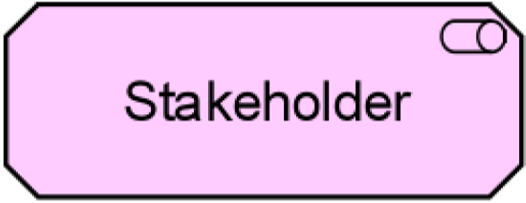
\includegraphics[scale=0.36,]			{imagenes/lenguaje/Motivational/stakeholder}}
		\\ \hline
		
		\begin{tabular}[c]{@{}c@{}}
			\\Conductor\\ (Driver)
		\end{tabular} 
		& Algo que crea, motiva y alimenta el cambio en una organización. 
		
		& \raisebox{-0,55\totalheight}{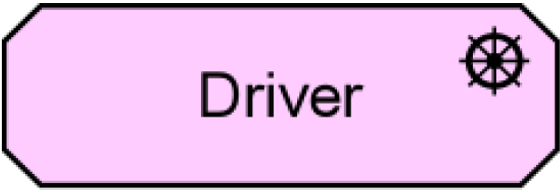
\includegraphics[scale=0.36,]			{imagenes/lenguaje/Motivational/driver}}
		\\ \hline
		
		\begin{tabular}[c]{@{}c@{}}
			\\Evaluación\\ (Assessment)
		\end{tabular}                  
		& El resultado de algunas evaluaciones de algunos conductores. 
		
		& \raisebox{-0,65\totalheight}{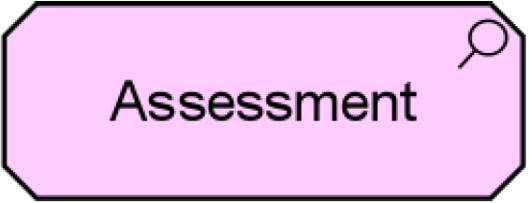
\includegraphics[scale=0.36,]			{imagenes/lenguaje/Motivational/assessment}}
		\\ \hline
		
		\begin{tabular}[c]{@{}c@{}}
			\\Gol\\ (Goal)
		\end{tabular}                      
		& Un estado final que una parte interesada desea lograr.    
		
		& \raisebox{-0,55\totalheight}{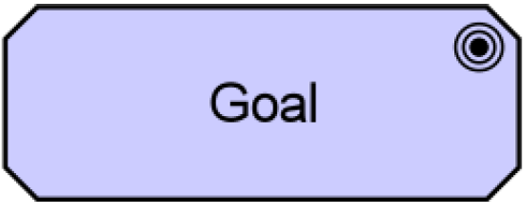
\includegraphics[scale=0.36,]			{imagenes/lenguaje/Motivational/goal}}
		\\ \hline
		
		\begin{tabular}[c]{@{}c@{}}
			\\Requisito\\ (Requirement)
		\end{tabular}                      
		&  Una declaración de necesidad que debe ser realizada por un sistema. 
		
		& \raisebox{-0,55\totalheight}{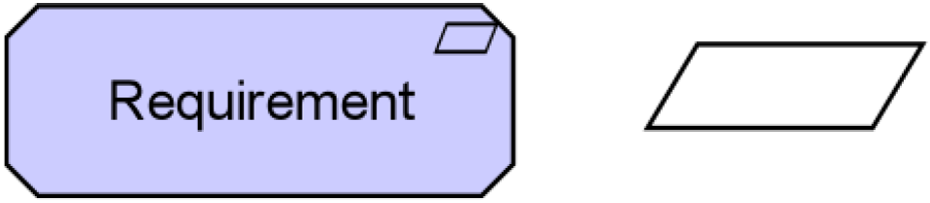
\includegraphics[scale=0.36,]			{imagenes/lenguaje/Motivational/requirement}}
		\\ \hline
		
		\begin{tabular}[c]{@{}c@{}}
			\\Restricción\\(Constraint)
		\end{tabular}                      
		& Una restricción de la forma en que se realiza un sistema.
		
		& \raisebox{-0,55\totalheight}{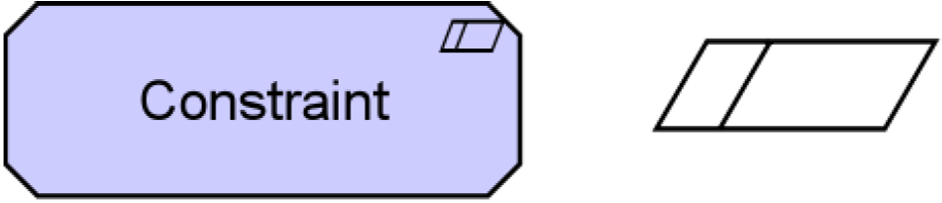
\includegraphics[scale=0.36,]			{imagenes/lenguaje/Motivational/constraint}}
		\\ \hline
		
		\begin{tabular}[c]{@{}c@{}}
			\\Principio\\ (Principle)
		\end{tabular}                      
		& Una propiedad normativa de todos los sistemas en un contexto dado, o la forma en que se realizan.                         
		& \raisebox{-0,66\totalheight}{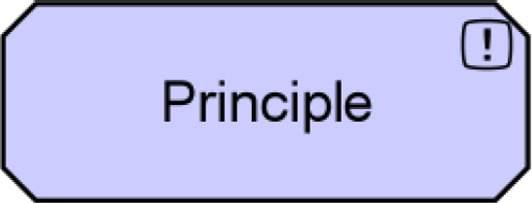
\includegraphics[scale=0.36,]			{imagenes/lenguaje/Motivational/principle}}
		\\ \hline
	\end{tabular}
	\caption{Capa de Motivación}
	\label{capaMotivacion}
\end{table}

\subsection{Resumen: capa de proyecto}
\begin{table}[H]
	
	\centering
	\begin{tabular}{|p{4cm}|p{5cm}|p{4cm}|}
		\hline
		\textbf{Concepto}                                                           & \multicolumn{1}{c|}{\textbf{Definición}}                                                             & \textbf{Notación} \\ \hline
		\begin{tabular}[c]{@{}c@{}}Paquete de Trabajo\\ (Work Package)\end{tabular} & Una serie de acciones diseñadas para lograr una meta única dentro de un tiempo especificado.         & 
		\raisebox{-\totalheight}{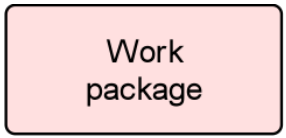
\includegraphics[scale=0.36,]			{imagenes/lenguaje/Proyect/WorkPackage.png}}
		\\ \hline
		\begin{tabular}[c]{@{}c@{}}Entregable\\ (Derivable)\end{tabular}            & Un resultado definido con precisión de un paquete de trabajo (work package).                         & 
		\raisebox{-\totalheight}{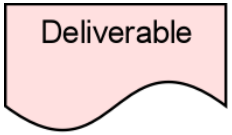
\includegraphics[scale=0.36,]			{imagenes/lenguaje/Proyect/Deliverable.png}}
		\\ \hline
		\begin{tabular}[c]{@{}c@{}}Meseta\\ (Plateau)\end{tabular}                  & Un estado relativamente estable de la arquitectura que existe durante un período de tiempo limitado. &  
		\raisebox{-\totalheight}{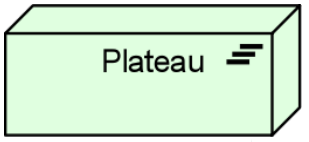
\includegraphics[scale=0.36,]			{imagenes/lenguaje/Proyect/Plateau.png}}
		\\ \hline
		\begin{tabular}[c]{@{}c@{}}Brecha\\ (Gap)\end{tabular}                      & Resultado de un análisis de la brecha entre dos mesetas (plateaus).                                  &  
		\raisebox{-\totalheight}{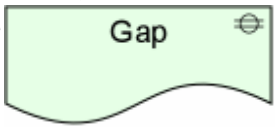
\includegraphics[scale=0.36,]			{imagenes/lenguaje/Proyect/Gap.png}}
		\\ \hline
	\end{tabular}
	\caption{Capa de Proyecto}
	\label{capa-proyecto}
\end{table}


\subsection{Resumen: capa de tecnologia}
\begin{center}
\begin{longtable}[H]{| >{\centering\arraybackslash}m{3cm} | >{\arraybackslash}m{6cm} | p{4cm} | p{5cm} | p{4cm} |}
	
		\hline
		\textbf{Concepto} &  \centering \textbf{Definición} & \textbf{Notación} \\
		\hline
		\endfirsthead
		
		
		\hline
		\textbf{Concepto} &  \centering \textbf{Definición} & \textbf{Notación} \\
		\hline
		\endhead
		
		Nodo        
		& \vspace{1mm} Un recurso computacional sobre el cual 
		los artefactos pueden ser almacenados o
		desplegados para su ejecución.        
		&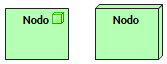
\includegraphics[width=30mm,trim=0 0 0 -2mm]{imagenes/lenguaje/tecnologia/nodo}  \\ \hline
		
		Dispositivo 
		& \vspace{1mm} Un recurso de hardware en el que los
		artefactos se pueden almacenar o desplegar 
		para su ejecución.              
		& 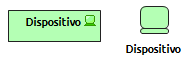
\includegraphics[width=35mm,trim=0 0 0 -2mm]{imagenes/lenguaje/tecnologia/dispositivo}  \\ \hline
		
		Red         
		&\vspace{1mm} Un medio de comunicación entre dos o
		más dispositivos.               
		& 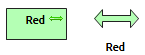
\includegraphics[width=25mm,trim=0 0 0 -2mm]{imagenes/lenguaje/tecnologia/red}  \\ \hline
		
		Ruta de 
		Comunicación	
		& \vspace{1mm} Un enlace entre dos o más nodos, a
		través del cual estos nodos pueden 
		intercambiar datos.                
		& 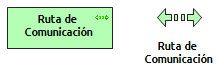
\includegraphics[width=35mm,trim=0 0 0 -2mm]{imagenes/lenguaje/tecnologia/comunicacion}  \\ \hline
		
		Interfaz de 
		infraestructura &\vspace{1mm} Un punto de acceso donde los servicios
		de infraestructura ofrecidos por un nodo 
		pueden ser accedidos por otros nodos y 
		componentes de la aplicación.
		&  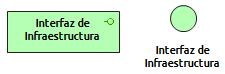
\includegraphics[width=35mm,trim=0 0 0 -2mm]{imagenes/lenguaje/tecnologia/interfaz}  \\ \hline
		
		Software del  
		Sistema
		&\vspace{1mm} Un entorno de software para tipos específicos de componentes y objetos que
		se despliegan en él en forma de artefactos.
		& 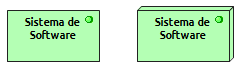
\includegraphics[width=35mm,trim=0 0 0 -2mm]{imagenes/lenguaje/tecnologia/software}  \\ \hline 
		
		Función de 
		Infraestructura 
		&\vspace{1mm} Un elemento de comportamiento que agrupa el comportamiento de infraes
		tructura que puede ser realizado por un	nodo.
		& 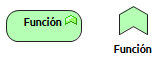
\includegraphics[width=35mm,trim=0 0 0 -2mm]{imagenes/lenguaje/tecnologia/funcion}  \\ \hline 	
		
		Servicio de 
		Infraestructura 
		&\vspace{1mm} Una unidad de funcionalidad visible externamente, proporcionada por uno o más nodos, expuesta a través de interfaces bien definidas y significativa para el entorno.
		&  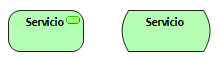
\includegraphics[width=35mm,trim=0 0 0 -2mm]{imagenes/lenguaje/tecnologia/servicio} \\ \hline 
		
		Artefacto 
		&\vspace{1mm} Una pieza física de datos que se utiliza ose produce en un proceso de desarrollo de software, o mediante el despliegue y la operación de un sistema. 
		& 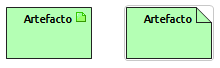
\includegraphics[width=35mm,trim=0 0 0 -2mm]{imagenes/lenguaje/tecnologia/artefacto}  \\ \hline
		

	\caption{Conceptos de Capa de Tecnología}
	
\end{longtable}
\end{center}


\subsection{Resumen Relaciones}

\subsubsection{Relaciones Estructurales}
\begin{center}
	\begin{longtable}[H]{| >{\centering\arraybackslash}m{3cm} | >{\arraybackslash}m{6cm} | p{4cm} | p{5cm} | p{4cm} |}
		
		\hline
		\textbf{Concepto} &  \centering \textbf{Definición} & \textbf{Notación} \\
		\hline
		\endfirsthead
		
		
		\hline
		\textbf{Concepto} &  \centering \textbf{Definición} & \textbf{Notación} \\
		\hline
		\endhead
		
		Asociacion       
		& \vspace{1mm} La asociación modela una relación entre
		objetos que no están cubiertos por otra más
		relación específica.        
		&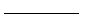
\includegraphics[width=30mm,trim=0 0 0 -2mm]{imagenes/lenguaje/relaciones/asociacion}  \\ \hline
		
		Acceso
		& \vspace{1mm} La relación de acceso modela el acceso de
		Conceptos conductuales para negocios o datos
		objetos.            
		& 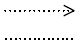
\includegraphics[width=35mm,trim=0 0 0 -2mm]{imagenes/lenguaje/relaciones/acceso}  \\ \hline
		
		Usado por        
		&\vspace{1mm} El utilizado por la relación modela el uso de
		servicios por procesos, funciones o
		interacciones y el acceso a las interfaces por
		roles, componentes o colaboraciones.               
		& \includegraphics[width=25mm,trim=0 0 0 -2mm]{imagenes/lenguaje/relaciones/usadopor}  \\ \hline
		
		Realización	
		& \vspace{1mm} La relación de realización vincula una lógica
		entidad con una entidad más concreta que
		se da cuenta.              
		& \includegraphics[width=35mm,trim=0 0 0 -2mm]{imagenes/lenguaje/relaciones/realizacion}  \\ \hline
		
		Asignación &\vspace{1mm} La relación de asignación vincula unidades de
		comportamiento con elementos activos (por ejemplo, roles,
		componentes) que los realizan, o roles con
		actores que los cumplen. 
		&  \includegraphics[width=35mm,trim=0 0 0 -2mm]{imagenes/lenguaje/relaciones/asignacion}  \\ \hline
		
		Agregacion
		&\vspace{1mm}  La relación de agregación indica que un
		el objeto agrupa varios otros objetos.
		& \includegraphics[width=35mm,trim=0 0 0 -2mm]{imagenes/lenguaje/relaciones/agregacion}  \\ \hline 
		
		Composición 
		&\vspace{1mm} La relación de composición indica que
		un objeto se compone de uno o más
		objetos.
		& \includegraphics[width=35mm,trim=0 0 0 -2mm]{imagenes/lenguaje/relaciones/composicion}  \\ \hline 			
		
		\caption{Conceptos de Capa de Relaciones Estructurales}
		
	\end{longtable}
\end{center}

\subsubsection{Relaciones Dinámicas}
\begin{center}
	\begin{longtable}[H]{| >{\centering\arraybackslash}m{3cm} | >{\arraybackslash}m{6cm} | p{4cm} | p{5cm} | p{4cm} |}
		
		\hline
		\textbf{Concepto} &  \centering \textbf{Definición} & \textbf{Notación} \\
		\hline
		\endfirsthead
		
		
		\hline
		\textbf{Concepto} &  \centering \textbf{Definición} & \textbf{Notación} \\
		\hline
		\endhead
		
		Flujo      
		& \vspace{1mm} La relación de flujo describe el intercambio
		o transferencia de, por ejemplo, información o
		valor entre procesos, función,
		interacciones y eventos.       
		&\includegraphics[width=30mm,trim=0 0 0 -2mm]{imagenes/lenguaje/relaciones/flujo}  \\ \hline
		
		Desencadenante
		& \vspace{1mm} La relación de activación describe el
		relaciones temporales o causales entre
		procesos, funciones, interacciones y eventos.  
		& \includegraphics[width=35mm,trim=0 0 0 -2mm]{imagenes/lenguaje/relaciones/triggering}  \\ \hline
		
		\caption{Conceptos de Capa de Relaciones Dinámicas}
		
	\end{longtable}
\end{center}

\subsubsection{Otras Relaciones}
\begin{center}
	\begin{longtable}[H]{| >{\centering\arraybackslash}m{3cm} | >{\arraybackslash}m{6cm} | p{4cm} | p{5cm} | p{4cm} |}
		
		\hline
		\textbf{Concepto} &  \centering \textbf{Definición} & \textbf{Notación} \\
		\hline
		\endfirsthead
		
		
		\hline
		\textbf{Concepto} &  \centering \textbf{Definición} & \textbf{Notación} \\
		\hline
		\endhead
		
		Agrupamiento     
		& \vspace{1mm} La relación de agrupamiento indica que
		objetos del mismo tipo o tipos diferentes
		pertenecen juntos basados en algunos
		característica.   
		&\includegraphics[width=15mm,trim=0 0 0 -2mm]{imagenes/lenguaje/relaciones/agrupacion}  \\ \hline
		
		Union
		& \vspace{1mm} Un cruce se usa para conectar relaciones de
		el mismo tipo
		& \includegraphics[width=10mm,trim=0 0 0 -2mm]{imagenes/lenguaje/relaciones/union}  \\ \hline
		
		
		
		Especialización
		& \vspace{1mm}La relación de especialización indica que
		un objeto es una especialización de otro objeto.
		& \includegraphics[width=35mm,trim=0 0 0 -2mm]{imagenes/lenguaje/relaciones/especializacion}  \\ \hline
		
		
		\caption{Conceptos de Capa de Relaciones Dinámicas}
		
	\end{longtable}
\end{center}

\chapter{Negocio}

\section{Introducción}
En esta capa se busca dar información acerca de una serie  de conceptos informativos para dar relevancia  en el dominio empresarial: un producto y contrato asociado, el significado de los objetos de negocio y el valor de los productos y servicios empresariales.\\
Para ello es necesario el diseño de 6 puntos de vista dentro de los cuales se encuentran: de organización, de cooperación de actor, de función de negocio, de proceso de negocio, de cooperación de proceso de negocio y de producto.\\
Los puntos de vista se mostrarán en dos partes, la primera de ellas será el modelo donde se encontrará una descripción del punto de vista acompañado de una tabla con la información de este y el meta-modelo correspondiente, en la segunda parte se encontrará el caso de estudio, es decir, el modelo donde será aplicado el meta-modelo previamente visto al proyecto y la organización en la que se está trabajando.
\newpage

\section{Punto de Vista de Organización}
\subsection{Descripción}
El punto de vista organizacional en la organización de la compañía, departamento, red de compañías, u otra identidad organizacional. Esto es posible para presentar modelos en este punto de vista como diagramas de bloques anidados, pero en el camino mas tradicional, tal como mapas organizacionales. El punto de vista organizacional es muy tratado en 	la identificación de competencias, autoridades y responsables en la organización.

\subsubsection{Metamodelo}
\begin{figure}[H]
	\centering
	\includegraphics[width=1.0\textwidth]{imagenes/Metamodelos/Negocio/meta_organizacion.PDF}
	\caption{Metamodelo: Punto de Vista de Organización}
	\label{fig:gap_analysis}
\end{figure}

\subsubsection{Caso de Estudio}
En el siguiente punto de vista podemos resaltar la sucursal como localización principal de la organización; adicionalmente, se puede observar la participación de actores quienes son los pilares fundamentales para la realización de los principales procesos en la compañía. Estos son: Seguridad y Administración.

\begin{figure}[H]
	\centering
	\includegraphics[width=1.0\textwidth]{imagenes/Caso_estudio/Negocio/Organizacion.PDF}
	\caption{Caso de estudio: Punto de Vista de Organización}
	\label{fig:gap_analysis}
\end{figure}




\section{Punto de Vista de Cooperación de Actor}
\subsection{Descripción}
El punto de vista de Cooperación de actor se enfoca en las relaciones que se presentan entre un actor y su entorno, se puede decir que es un diagrama de contexto en el cual se coloca la organización en su entorno, además de esto se puede evidenciar clientes, proveedores y compañeros de negocio, tiene como objetivo determinar dependencias y colaboraciones externas y ver la relación con los actores que se encuentran en este diagrama, tenemos por otra parte que en este punto de vista se puede evidenciar el número de actores cooperantes  de negocio van a tener participación en esta capa o cuantos componentes de aplicación interactúan para formar un proceso de negocio.

\subsubsection{Metamodelo}
\begin{figure}[H]
	\centering
	\includegraphics[width=1.0\textwidth]{imagenes/Metamodelos/Negocio/meta_cooperacion_actor.png}
	\caption{Metamodelo: Punto de Vista de Organización}
	\label{fig:gap_analysis}
\end{figure}




\subsubsection{Caso de Estudio}
La colaboración Espacio de Parqueadero, surge de la interacción de los roles Sucursal y Clientes del Parqueadero. Por parte de la sucursal, brindando el terrero de parqueo; y por parte de los clientes, al realizar el uso del mismo a través de la interface que se encuentra de cara a ellos, la Recepción.
\begin{figure}[H]
	\centering
	\includegraphics[width=1.0\textwidth]{imagenes/Caso_estudio/Negocio/CopActor.PDF}
	\caption{Caso de estudio: Punto de Vista de Cooperación de Actor}
	\label{fig:gap_analysis}
\end{figure}










\section{Punto de Vista de Función de Negocio}
\subsection{Descripción}
El punto de vista Función de negocio muestra las principales funciones de negocio de una organización y sus relaciones en términos de los flujos de información, valor o bienes entre ellos. Las funciones empresariales se utilizan para representar los aspectos más estables de una empresa en términos de las actividades primarias que realiza, independientemente de los cambios organizacionales o desarrollos tecnológicos.

Por lo tanto, la arquitectura de la función comercial de las empresas que operan en el mismo mercado a menudo muestran similitudes cercanas. Por lo tanto, el punto de vista de la función empresarial proporciona una visión de alto nivel de las operaciones generales de la empresa y puede utilizarse para identificar las competencias necesarias o estructurar una organización de acuerdo con sus principales actividades.


\subsubsection{Metamodelo}
\begin{figure}[H]
	\centering
	\includegraphics[width=1.0\textwidth]{imagenes/Metamodelos/Negocio/meta_funcion_negocio.png}
	\caption{Metamodelo: Punto de Vista de Función de Negocio}
	\label{fig:gap_analysis}
\end{figure}



\subsubsection{Caso de Estudio}
En el siguiente punto de vista se resalta la presencia de los actores Operario y Jefe de Seguridad, quienes llevan a cabo funciones específicas de los roles de Operación y Seguridad, tales como: Registro de Ingreso, Asignación de Parqueadero, Registro de Usuarios, Registro de Pagos, Registro de Retiros y Verificación de propiedad del vehículo.

\begin{figure}[H]
	\centering
	\includegraphics[width=1.0\textwidth]{imagenes/Caso_estudio/Negocio/FunNegocio.PDF}
	\caption{Caso de estudio: Punto de vista de función de negocio.}
	\label{fig:gap_analysis}
\end{figure}








\section{Punto de Vista de Proceso de Negocio}
\subsection{Descripción}
El punto de vista de proceso de negocio es usado para ver la estructura desde un nivel alto además de esto de poder evidenciar la composición de uno o más procesos de negocio, dentro de este punto de vista podemos resaltar que se enfoca en los servicios que un proceso de negocio puede ofrecer al cliente mostrando como este proceso puede contribuir para la realización de productos, por otro lado se puede hacer una asociación en cuanto a responsabilidades que tienen los actores asociados y los roles dentro de este proceso de negocio y por último en este punto de vista podemos evidenciar la información utilizada por el proceso de negocio.

\subsubsection{Metamodelo}
\begin{figure}[H]
	\centering
	\includegraphics[width=1.0\textwidth]{imagenes/Metamodelos/Negocio/meta_proceso_negocio.png}
	\caption{Metamodelo: Punto de Vista de Proceso de Negocio}
	\label{fig:gap_analysis}
\end{figure}


\subsubsection{Caso de Estudio}
En este punto de vista podemos resaltar el proceso principal de la organización: Renta de espacio de parqueo, el cual es originado por una solicitud del espacio y finaliza en el retiro del vehículo. Dentro de este proceso tenemos los subprocesos de: Registro de Usuario, Registro de Ingreso, Asignación de Espacio, Vigilancia de Vehículo, Cálculo de tarifa y Registro de Pago.

\begin{figure}[H]
	\centering
	\includegraphics[width=1.0\textwidth]{imagenes/Caso_estudio/Negocio/ProNegocio.PDF}
	\caption{Caso de estudio: Punto de vista de proceso de negocio.}
	\label{fig:gap_analysis}
\end{figure}

\section{Punto de vista de Cooperación de procesos de negocio.}
\subsection{Descripción}
El punto de vista de Cooperación de Proceso de Negocio se utiliza para mostrar las relaciones de
uno o más procesos de negocio entre sí y / o con su entorno. Puede utilizarse tanto para crear un diseño
de alto nivel de procesos empresariales dentro de su contexto como para proporcionar un gestor
operativo responsable de uno o más de dichos procesos con información sobre sus dependencias

\subsubsection{Metamodelo}
\begin{figure}[H]
	\centering
	\includegraphics[width=1.0\textwidth]{imagenes/Metamodelos/Negocio/meta_cooperacion_proceso_negocio.png}
	\caption{Metamodelo: Punto de Vista de Cooperación de Negocio}
	\label{fig:gap_analysis}
\end{figure}



\subsubsection{Caso de Estudio}
Adicional al punto de vista anterior, se evidencian los roles involucrados, Administrador y Agente de Seguridad, en el proceso Renta de espacio de parqueo, para llevar a cabo el cumplimiento del servicio fundamental de la organización, Renta de espacio de parqueadero y vigilancia para bicicletas.

\begin{figure}[H]
	\centering
	\includegraphics[width=1.0\textwidth]{imagenes/Caso_estudio/Negocio/CoProNegocios.PDF}
	\caption{Caso de estudio: Punto de vista de colabroacion de procesos de negocio.}
	\label{fig:gap_analysis}
\end{figure}


\section{Punto de Vista de Producto}

\subsection{Descripción}
El punto de vista del producto representa el valor que ese producto ofrece a los clientes u otros involucrados y muestra la composición de uno o mas productos en términos de los servicios constituidos y la asociación de contratos u otros acuerdos. Esto también puede ser usado para mostrar los canales de interfaces que este producto ofrece, y los eventos asociados con el producto. Un punto de vista del producto es típicamente usado en el desarrollo del producto a el diseño del producto por la composición de servicios existentes o la identificación que nuevos servicios tiene que ser creados para este producto,dando el valor a las expectativas del cliente para este. Este puede servir para la entrada para la arquitectura del proceso de negocio y otros que necesiten diseñar el proceso y ICT realizan estos productos. 

\subsubsection{Metamodelo}
\begin{figure}[H]
	\centering
	\includegraphics[width=1.0\textwidth]{imagenes/Metamodelos/Negocio/meta_producto.png}
	\caption{Metamodelo: Punto de Vista de Prodcuto}
	\label{fig:gap_analysis}
\end{figure}


\subsubsection{Caso de Estudio}
El producto principal que ofrece la organización, como se evidencia en los puntos de vista anteriores, es el espacio de parqueo, el cual se caracteriza por proponer espacios adecuados y seguros para las bicicletas de los clientes, a la vez de ofrecer un servicio integral de vigilancia permanente para los vehículos, soportados por sus correspondientes procesos.
\begin{figure}[H]
	\centering
	\includegraphics[width=1.0\textwidth]{imagenes/Caso_estudio/Negocio/Producto.PDF}
	\caption{Caso de estudio: Punto de vista de producto}
	\label{fig:gap_analysis}
\end{figure}



\chapter{Aplicación}

\chapter{Capa de Aplicación}

\section{Introducción}
En esta capa de aplicaciones observaremos los principales conceptos de comunicación entre componentes por medio de interfaces, donde en los siguientes diagramas se pueden observar los principales comportamientos del aplicativo mediante 4 puntos de vista: Comportamiento de aplicación, Cooperación de aplicación, Estructura de aplicación y el uso de la aplicación.\\
Tal como mencionamos anteriormente, en nuestra capa de aplicación se caracteriza por poseer una arquitectura de componentes, de tal forma que  mostramos las principales funciones dentro de cada componente y ademas como se relacionan y comunican cada uno de estos, de tal forma que observemos como sera el comportamiento y la logica de la aplicación

\section{Punto de Vista de Comportamiento de Aplicación}
\subsection{Descripción}
El punto de vista de comportamiento de aplicación, describe el comportamiento interno de la aplicación, que este realiza uno o más servicios de aplicaciones. El punto de vista es útil en diseñar el principal comportamiento de la aplicación, o identificar superposición funcional entre diferentes aplicación.

\subsubsection{Metamodelo}
\begin{figure}[H]
	\centering
	\includegraphics[width=1.0\textwidth]{imagenes/Metamodelos/Aplicacion/meta_comportamiento_aplicacion.png}
	\caption{Metamodelo: Punto de Vista de Comportamiento de Aplicación.}
	\label{fig:gap_analysis}
\end{figure}

\subsubsection{Caso de Estudio}
En el presente caso de estudio, podemos observar el componente aplicación de la aplicación Two Wheels Digital, el cual se divide compone a su vez de componentes más pequeños como lo son Pagos, que se encarga de cumplir las funciones de cálculo de la tarifa y recepción del pago realizado por cada cliente. Por otra parte, el Gestor de Espacios encargado de la administración de los espacios de parqueo; el Gestor de Usuarios quien lleva a cabo el proceso de registro y validación. Por último, el componente de Estadísticas el cual elabora reportes sobre la renta de los espacios de parqueo.
\begin{figure}[H]
	\centering
	\includegraphics[width=1.0\textwidth]{imagenes/Caso_Estudio/Aplicacion/ComAplicacion.PDF}
	\caption{Caso de estudio: Punto de vista de comportamiento de aplicación.}
	\label{fig:gap_analysis}
\end{figure}




\section{Punto de Vista de Cooperación de Aplicación}
\subsection{Descripción}
El punto de vista Cooperación de aplicación describe las relaciones entre los componentes de la aplicaciones en términos de la información que se maneja entre ellos además de esto también se puede enfocar en términos de los servicios que estos ofrecen y de los que hacen uso. Este punto de vista también es usado para crear una visión general de todo el contexto de aplicación de una organización. Este punto de vista también es usado para expresar la cooperación interna de servicios que trabajando de una forma conjunta soportan la ejecución de un proceso de negocio.

\subsubsection{Metamodelo}
\begin{figure}[H]
	\centering
	\includegraphics[width=1.0\textwidth]{imagenes/Metamodelos/Aplicacion/meta_cooperacion_aplicacion.png}
	\caption{Metamodelo: Punto de Vista de Cooperación de Aplicación.}
	\label{fig:gap_analysis}
\end{figure}

\subsubsection{Caso de Estudio}
Por medio de este punto de vista, se resalta la arquitectura general de tres capas de la aplicación Two Wheels Digital en donde el componente principal de interfaz se encuentra ubicado en la capa de presentación; los componentes Gestor de Usuarios, Gestor de Espacios, Pagos y Estadísticas se ubican en la capa de negocio, y finalmente el componente de almacenamiento, Base de Datos, se ubica en la capa de persistencia.

\begin{figure}[H]
	\centering
	\includegraphics[width=1.0\textwidth]{imagenes/Caso_Estudio/Aplicacion/CoopAplicacion.PDF}
	\caption{Caso de estudio: Punto de vista de cooperación de aplicación.}
	\label{fig:gap_analysis}
\end{figure}






\section{Punto de Vista de Uso de Aplicación}
\subsection{Descripción}
El punto de vista Uso de aplicaciones describe cómo se utilizan las aplicaciones para soportar uno o más procesos empresariales y cómo se utilizan en otras aplicaciones. Se puede utilizar en el diseño de una aplicación mediante la identificación de los servicios necesarios por los procesos de negocio y otras aplicaciones, o en el diseño de procesos de negocio mediante la descripción de los servicios que están disponibles. Además, puesto que identifica las dependencias de los procesos de negocio en las aplicaciones, puede ser útil para los gerentes operacionales responsables de estos procesos.

\subsubsection{Metamodelo}
\begin{figure}[H]
	\centering
	\includegraphics[width=1.0\textwidth]{imagenes/Metamodelos/Aplicacion/meta_uso_aplicacion.png}
	\caption{Metamodelo: Punto de Vista de Uso de Aplicación.}
	\label{fig:gap_analysis}
\end{figure}

\subsubsection{Caso de Estudio}
Se tiene como enfoque principal el proceso de Renta de espacios de parqueadero el cual hace uso de tres servicios llevados a cabo por el componente principal de la aplicación Two Wheels Digital, como lo son la gestión de usuarios, la gestión de espacios y la gestión de pagos.

\begin{figure}[H]
	\centering
	\includegraphics[width=1.0\textwidth]{imagenes/Caso_Estudio/Aplicacion/UsoAplicacion.PDF}
	\caption{Caso de estudio: Punto de vista de Uso de aplicación.}
	\label{fig:gap_analysis}
\end{figure}

\section{Punto de vista de Estructura de Aplicación}
\subsection{Descripción}
El punto de vista de Estructura de la aplicación muestra la estructura de una o más aplicaciones
o componentes. Este punto de vista es útil para diseñar o comprender la estructura principal de
aplicaciones o componentes y los datos asociados, por ejemplo, para descomponer la estructura del
sistema en construcción o para identificar componentes de aplicación heredados que son adecuados
para la migración/integración.

\subsubsection{Metamodelo}
\begin{figure}[H]
	\centering
	\includegraphics[width=1.0\textwidth]{imagenes/Metamodelos/Aplicacion/meta_estructura_aplicacion.png}
	\caption{Metamodelo: Punto de Vista de Estructura de Aplicación.}
	\label{fig:gap_analysis}
\end{figure}

\subsubsection{Caso de Estudio}

\begin{figure}[H]
	\centering
	\includegraphics[width=1.0\textwidth]{imagenes/Caso_Estudio/Aplicacion/EstAplicacion.PDF}
	\caption{Caso de estudio: Punto de vista de estructura de aplicación.}
	\label{fig:gap_analysis}
\end{figure}

\chapter{Tecnología}

\chapter{Capa de Tecnologia}

\section{Introducción}
En esta capa de aplicaciones observaremos los principales conceptos de comunicación entre componentes por medio de interfaces, donde en los siguientes diagramas se pueden observar los principales comportamientos del aplicativo mediante 4 puntos de vista: Comportamiento de aplicación, Cooperación de aplicación, Estructura de aplicación y el uso de la aplicación.\\
Tal como mencionamos anteriormente, en nuestra capa de aplicación se caracteriza por poseer una arquitectura de componentes, de tal forma que  mostramos las principales funciones dentro de cada componente y ademas como se relacionan y comunican cada uno de estos, de tal forma que observemos como sera el comportamiento y la logica de la aplicación

\section{Punto de Vista de Infraestructura}
\subsection{Descripción}
El punto de vista de infraestructura contiene los elementos de hardware y de software correspondientes a la infraestructura que soporta la capa de aplicación, en este diagrama podemos observar elementos ales como dispositivos físicos, redes o sistemas de software tales como: Bases de datos o sistemas operativos.

\subsubsection{Caso de Estudio}


\begin{figure}[H]
	\centering
	\includegraphics[width=1.0\textwidth]{imagenes/Caso_Estudio/Tecnologia/ComAplicacion.PDF}
	\caption{Caso de estudio: Punto de vista de Infraesructura.}
	\label{fig:gap_analysis}
\end{figure}

\section{Punto de Vista de Uso de Infraestructura}
\subsection{Descripción}
El punto de vista de Uso de Infraestructura muestra como las aplicaciones están soportadas por una infraestructura de hardware y software en la que los servicios de infraestructura  son ofrecidos por los dispositivos mientras que las  redes y los sistemas de software proporcionan las aplicaciones. Este punto de vista juega un papel importante en el análisis del rendimiento y la escalabilidad, ya que relaciona la infraestructura física con el mundo lógico de las aplicaciones. Es muy útil para determinar el rendimiento y los requisitos de calidad en la infraestructura en función de las demandas de las distintas aplicaciones que lo utilizan.

\subsubsection{Metamodelo}
\begin{figure}[H]
	\centering
	\includegraphics[width=1.0\textwidth]{imagenes/Metamodelos/Tecnologia/Estructura_informacion.PDF}
	\caption{Metamodelo: Punto de Vista de Uso de Infraestrucutra.}
	\label{fig:gap_analysis}
\end{figure}


\subsubsection{Caso de Estudio}


\begin{figure}[H]
	\centering
	\includegraphics[width=1.0\textwidth]{imagenes/Caso_Estudio/Tecnologia/ComAplicacion.PDF}
	\caption{Caso de estudio: Punto de vista de Uso de Infraesructura.}
	\label{fig:gap_analysis}
\end{figure}


\section{Punto de Vista de Organización e implementación}
\subsection{Descripción}
El punto de vista de organización e implementación muestra como se implementan una o mas aplicaciones o componentes en la insfraestructura. Esto se comprende como el mapeo de aplicaciones lógicas a su respectivos componente o artefacto físico, de igual manera se puede evidenciar un mapeo de  la información que utilizan estas.

\subsubsection{Metamodelo}
\begin{figure}[H]
	\centering
	\includegraphics[width=1.0\textwidth]{imagenes/Metamodelos/Tecnologia/Estructura_informacion.PDF}
	\caption{Metamodelo: Punto de Vista de Organización e Implementación.}
	\label{fig:gap_analysis}
\end{figure}

\subsubsection{Caso de Estudio}


\begin{figure}[H]
	\centering
	\includegraphics[width=1.0\textwidth]{imagenes/Caso_Estudio/Tecnologia/ComAplicacion.PDF}
	\caption{Caso de estudio: Punto de Vista de Organización e implementación.}
	\label{fig:gap_analysis}
\end{figure}


\section{Punto de Vista de Estructura de Información}
\subsection{Descripción}
El punto de vista de la estructura de información muestra la estructura de la información utilizada en la: empresa, proceso o una aplicación comercial específica; esto en términos de tipos de datos o estructuras de clases (orientadas a objetos). Además, puede mostrar cómo la información se representa en el nivel de negocio, en el nivel de aplicación mediante las estructuras de datos utilizadas allí, y cómo estas se asignan a la infraestructura subyacente mediante artefactos.

\subsubsection{Metamodelo}
\begin{figure}[H]
	\centering
	\includegraphics[width=1.0\textwidth]{imagenes/Metamodelos/Tecnologia/Estructura_informacion.PDF}
	\caption{Metamodelo: Punto de Vista de Estructura de Información.}
	\label{fig:gap_analysis}
\end{figure}

\subsubsection{Caso de Estudio}


\begin{figure}[H]
	\centering
	\includegraphics[width=1.0\textwidth]{imagenes/Caso_Estudio/Tecnologia/ComAplicacion.PDF}
	\caption{Caso de estudio: Punto de Vista de Estructura de información.}
	\label{fig:gap_analysis}
\end{figure}


\section{Punto de Vista de Realización del Servicio}
\subsection{Descripción}
El punto de vista de Realización del servicio se utiliza para mostrar cómo uno o más servicios de negocio se realizan mediante los procesos subyacentes (y, en ocasiones, mediante los componentes de la aplicación). Por lo tanto, forma el puente entre el punto de vista del producto y la vista del proceso de negocios. Proporciona una "vista desde el exterior" en uno o más procesos comerciales.

\subsubsection{Metamodelo}
\begin{figure}[H]
	\centering
	\includegraphics[width=1.0\textwidth]{imagenes/Metamodelos/Tecnologia/Estructura_informacion.PDF}
	\caption{Metamodelo: Punto de Vista de Realización del Servicio.}
	\label{fig:gap_analysis}
\end{figure}

\subsubsection{Caso de Estudio}

\begin{figure}[H]
	\centering
	\includegraphics[width=1.0\textwidth]{imagenes/Caso_Estudio/Tecnologia/ComAplicacion.PDF}
	\caption{Caso de estudio: Punto de Vista de Realizacion del Servicio.}
	\label{fig:gap_analysis}
\end{figure}


\section{Punto de Vista de Capas}
\subsection{Descripción}
El punto de vista en capas representa varias capas y aspectos de una arquitectura empresarial en un diagrama. El principio estructural detrás de un punto de vista completamente estratificado es que cada capa dedicada expone, mediante la relación de "realización", una capa de servicios, que luego son "utilizados por" la siguiente capa dedicada. Por lo tanto, podemos separar fácilmente la estructura interna y la organización de una capa dedicada de su comportamiento externo observable expresado como la capa de servicio que la capa dedicada realiza.  El objetivo principal del punto de vista de capas es proporcionar información general en un diagrama.

\subsubsection{Metamodelo}
\begin{figure}[H]
	\centering
	\includegraphics[width=1.0\textwidth]{imagenes/Metamodelos/Tecnologia/Estructura_informacion.PDF}
	\caption{Metamodelo: Punto de Vista de Uso de capas.}
	\label{fig:gap_analysis}
\end{figure}

\subsubsection{Caso de Estudio}


\begin{figure}[H]
	\centering
	\includegraphics[width=1.0\textwidth]{imagenes/Caso_Estudio/Tecnologia/ComAplicacion.PDF}
	\caption{Caso de estudio: Punto de Vista de Capas.}
	\label{fig:gap_analysis}
\end{figure}


\chapter{Motivación}


\section{Introducción}
En las capas anteriores hemos visto como la estructura tecnológica le da soporte a la arquitectura empresarial, pero en esta capa vamos a visualizar y a modelar las razones o motivaciones que subyacen al diseño de esta, ya que son estas motivaciones las que restringen y van guiando el diseño de esta.
Las motivaciones reales están representadas por metas, principios, requisitos y restricciones.Las metas buscan representar algún resultado deseado - o fin - que una parte interesada desea lograr; por ejemplo, aumentar la satisfacción del cliente. 
Los principios y requisitos representan las propiedades deseadas de soluciones  o medios  mediante los cuales se pueden alcanzar los objetivos. 
Los principios son una serie de normativas  o pautas que guían el diseño de todas las soluciones posibles en un contexto dado. Y finalmente los requisitos representan declaraciones formales de necesidad, expresada por las partes interesadas, que debe cumplir la arquitectura o las soluciones siendo estas últimas inamovibles.


\section{Punto de Vista de StakeHolder}
\subsection{Descripción}
El punto de vista de infraestructura contiene los elementos de hardware y de software correspondientes a la infraestructura que soporta la capa de aplicación, en este diagrama podemos observar elementos ales como dispositivos físicos, redes o sistemas de software tales como: Bases de datos o sistemas operativos.

\subsubsection{Metamodelo}
\begin{figure}[H]
	\centering
	\includegraphics[width=1.0\textwidth]{imagenes/Metamodelos/Motivacion/meta_Stakeholder.pdf}
	\caption{Metamodelo: Punto de Vista de StakeHolder}
	\label{fig:gap_analysis}
\end{figure}

\subsubsection{Caso de Estudio}


\begin{figure}[H]
	\centering
	\includegraphics[width=1.0\textwidth]{imagenes/Caso_Estudio/Motivacion/Stakeholder.PDF}
	\caption{Caso de estudio: Punto de Vista de StakeHolder.}
	\label{fig:gap_analysis}
\end{figure}



\section{Punto de Vista de Realización de Objetivos}
\subsection{Descripción}

\subsubsection{Metamodelo}
\begin{figure}[H]
	\centering
	\includegraphics[width=1.0\textwidth]{imagenes/Metamodelos/Motivacion/meta_Realizacion_Objetivos.pdf}
	\caption{Metamodelo: Punto de Vista de Realización de Objetivos}
	\label{fig:gap_analysis}
\end{figure}

\subsubsection{Caso de Estudio}


\begin{figure}[H]
	\centering
	\includegraphics[width=1.0\textwidth]{imagenes/Caso_Estudio/Motivacion/Realizacion_Objetivos.PDF}
	\caption{Caso de estudio: Punto de Vista de Realización de Objetivos.}
	\label{fig:gap_analysis}
\end{figure}

\section{Punto de Vista de Contribución}
\subsection{Descripción}

\subsubsection{Metamodelo}
\begin{figure}[H]
	\centering
	\includegraphics[width=1.0\textwidth]{imagenes/Metamodelos/Motivacion/meta_Contribucon.pdf}
	\caption{Metamodelo: Punto de Vista de Contribución.}
	\label{fig:gap_analysis}
\end{figure}

\subsubsection{Caso de Estudio}


\begin{figure}[H]
	\centering
	\includegraphics[width=1.0\textwidth]{imagenes/Caso_Estudio/Motivacion/Contribucion.PDF}
	\caption{Caso de estudio: Punto de Vista de Contribución.}
	\label{fig:gap_analysis}
\end{figure}

\section{Punto de Vista de Principios}
\subsection{Descripción}

\subsubsection{Metamodelo}
\begin{figure}[H]
	\centering
	\includegraphics[width=1.0\textwidth]{imagenes/Metamodelos/Motivacion/meta_Principios.pdf}
	\caption{Metamodelo: Punto de Vista de Principios.}
	\label{fig:gap_analysis}
\end{figure}

\subsubsection{Caso de Estudio}


\begin{figure}[H]
	\centering
	\includegraphics[width=1.0\textwidth]{imagenes/Caso_Estudio/Motivacion/Principios.PDF}
	\caption{Caso de estudio: Punto de Vista de Principios.}
	\label{fig:gap_analysis}
\end{figure}

\section{Punto de Vista de Realización de Requerimientos}
\subsection{Descripción}

\subsubsection{Metamodelo}
\begin{figure}[H]
	\centering
	\includegraphics[width=1.0\textwidth]{imagenes/Metamodelos/Motivacion/meta_Realizacion_Requerimientos.pdf}
	\caption{Metamodelo: Punto de Vista de Realización de Requerimientos.}
	\label{fig:gap_analysis}
\end{figure}

\subsubsection{Caso de Estudio}


\begin{figure}[H]
	\centering
	\includegraphics[width=1.0\textwidth]{imagenes/Caso_Estudio/Motivacion/Realizacion_Requerimientos.PDF}
	\caption{Caso de estudio: Punto de Vista de Realización de Requerimientos.}
	\label{fig:gap_analysis}
\end{figure}


\section{Punto de Vista de Motivación}
\subsection{Descripción}

\subsubsection{Metamodelo}
\begin{figure}[H]
	\centering
	\includegraphics[width=1.0\textwidth]{imagenes/Metamodelos/Motivacion/meta_Motivacion.pdf}
	\caption{Metamodelo: Punto de Vista de Motivación.}
	\label{fig:gap_analysis}
\end{figure}

\subsubsection{Caso de Estudio}


\begin{figure}[H]
	\centering
	\includegraphics[width=1.0\textwidth]{imagenes/Caso_Estudio/Motivacion/Motivacion.PDF}
	\caption{Caso de estudio: Punto de Vista de Motivación.}
	\label{fig:gap_analysis}
\end{figure}



\chapter{Migración}


\section{Introducción}

\section{Punto de Vista de Proyecto}
\subsection{Descripción}

\subsubsection{Metamodelo}
\begin{figure}[H]
	\centering
	\includegraphics[width=1.0\textwidth]{imagenes/Metamodelos/Migracion/meta_Proyecto.pdf}
	\caption{Metamodelo: Punto de Vista de Proyecto.}
	\label{fig:gap_analysis}
\end{figure}

\subsubsection{Caso de Estudio}


\begin{figure}[H]
	\centering
	\includegraphics[width=1.0\textwidth]{imagenes/Caso_Estudio/Migracion/Proyecto.PDF}
	\caption{Caso de estudio: Punto de Vista de Proyecto.}
	\label{fig:gap_analysis}
\end{figure}

\section{Punto de Vista de Migración}
\subsection{Descripción}


\subsubsection{Metamodelo}
\begin{figure}[H]
	\centering
	\includegraphics[width=1.0\textwidth]{imagenes/Metamodelos/Migracion/meta_Migracion.pdf}
	\caption{Metamodelo: Punto de Vista de Migración}
	\label{fig:gap_analysis}
\end{figure}

\subsubsection{Caso de Estudio}


\begin{figure}[H]
	\centering
	\includegraphics[width=1.0\textwidth]{imagenes/Caso_Estudio/Migracion/Migracion.PDF}
	\caption{Caso de estudio: Punto de Vista de Migración.}
	\label{fig:gap_analysis}
\end{figure}

\section{Punto de Vista de Migración e Implementación}
\subsection{Descripción}


\subsubsection{Metamodelo}
\begin{figure}[H]
	\centering
	\includegraphics[width=1.0\textwidth]{imagenes/Metamodelos/Migracion/meta_Migracion_implementacion.pdf}
	\caption{Metamodelo: Punto de Vista de Migración e Implementación.}
	\label{fig:gap_analysis}
\end{figure}

\subsubsection{Caso de Estudio}


\begin{figure}[H]
	\centering
	\includegraphics[width=1.0\textwidth]{imagenes/Caso_Estudio/Migracion/Migracion_Implementacion.PDF}
	\caption{Caso de estudio: Punto de Vista de Migración e Implementación.}
	\label{fig:gap_analysis}
\end{figure}



\part{Diseño}
\chapter{Casos de USo}
\chapter{Interacciones}
\chapter{Clases}
\chapter{Estados}
\chapter{Actividades}
\chapter{Sistemas}
\chapter{Componentes}
\chapter{Nodos}

\chapter{Patrones GoF}

\part{Reflexiones}
\chapter{Conclusiones y Trabajos futuros}
\include{reflexiones/trabajos futuros}
\chapter*{Anexos}

\backmatter
% bibliography, glossary and index would go here.
\bibliographystyle{plain}
\bibliography{bibliografia/libros,bibliografia/articulos}

\end{document}